\documentclass[paper=A4,12pt,pagesize,twoside,BCOR=8mm,ngerman]{scrartcl}
\usepackage[utf8]{inputenc} 
\usepackage[T1]{fontenc}
\usepackage[ngerman]{babel}
\usepackage{lmodern}
\usepackage{microtype}

\usepackage{amsmath}
\usepackage{amsfonts}
\usepackage{siunitx}
\usepackage{graphicx}
\usepackage{caption}
\usepackage{textcomp}
\usepackage{pdfpages}
\usepackage{tikz}
\usepackage{float}
\usepackage{fancyhdr}
\usepackage{nicefrac}
\usepackage{tabularx}

\renewcommand{\v}[1]{\ensuremath{\mathbf{#1}}} % for vectors
\newcommand{\gv}[1]{\ensuremath{\mbox{\boldmath$ #1 $}}} 
\newcommand{\abs}[1]{\left| #1 \right|} % for absolute value
\newenvironment{rcases}{% 
  \left.\renewcommand*\lbrace.% 
  \begin{cases}}% 
{\end{cases}\right\rbrace}


\usepackage{booktabs, dcolumn, multirow}

\makeatletter
\newcolumntype{d}[1]{
>{\DC@{.}{,}{#1}}l<{\DC@end}
}
\makeatother

\pagestyle{headings}

\title{\textnormal{Scriptum}\\ Moderne Experimentalphysik \uppercase\expandafter{\romannumeral2\relax}\\\textnormal{\large{gelesen von Martin Wegener WS2013/14}}}
\author{}
\date{}

\setlength{\parindent}{0pt}

\begin{document}
\maketitle
\vfill
\begin{center}
	\large{Ge\TeX t von J. Müller}
\end{center}
\setcounter{page}{0} 
\thispagestyle{empty}
\newpage
\tableofcontents
\newpage
\marginpar {22.10.2013}
\section{Kristalline, quasikristalline und amorphe Festkörper}
	\subsection{Das periodische Gitter im Ortraum}
		\subsubsection{Einführung}
			\begin{figure}[H]
				\centering
				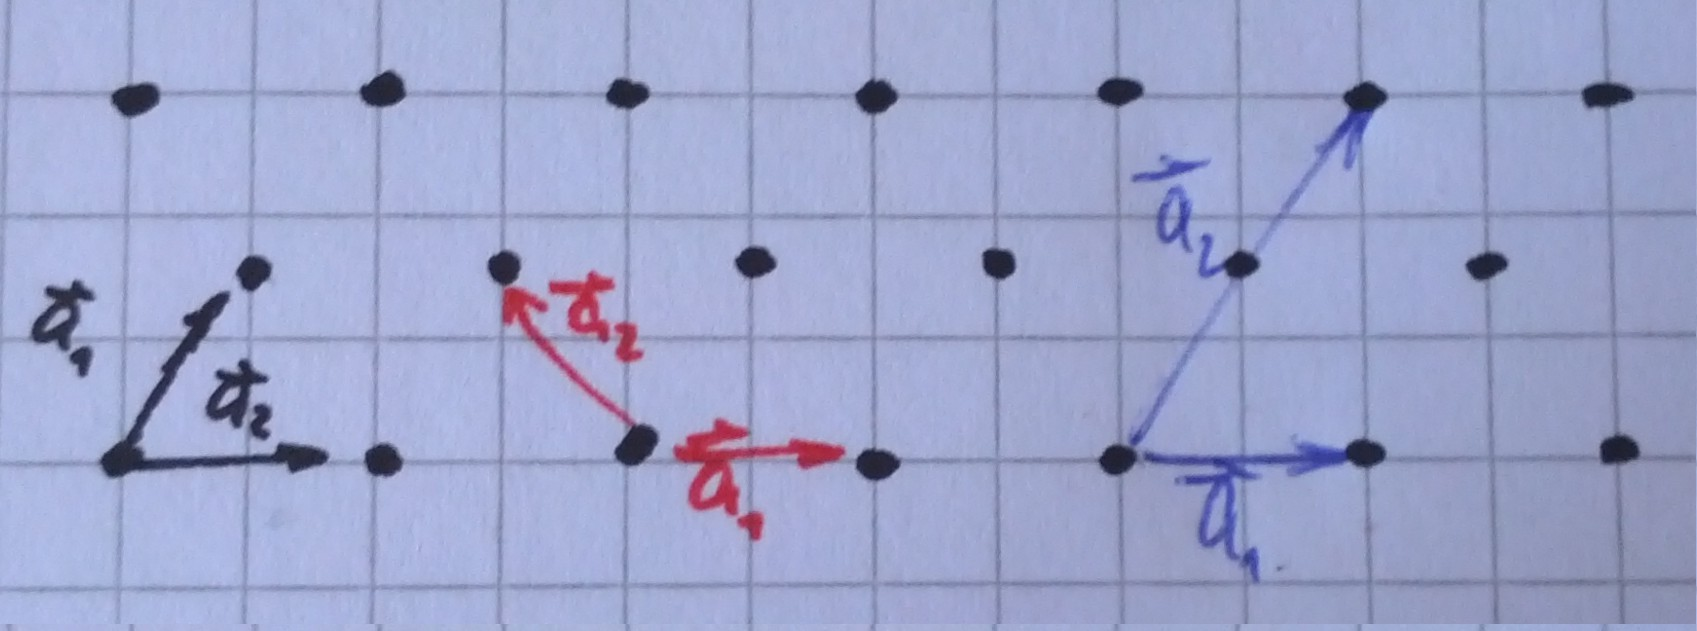
\includegraphics[width=0.6\textwidth]{pics/pic001.jpg}
				%\caption{Vektoren zwischen Gitterpunkten}
			\end{figure}
					
\marginpar {24.10.2013}

			d.h. von den Punkten $\vec{r}$, $\vec{r}\, '$ sieht das 
			Gitter gleich aus wenn gilt
			\begin{center}
			\fbox{$\vec{r}\, ' = \underbrace{\vec{r} + u \vec{a_1} + 
			v \vec{a_2} + w \vec{a_3}}_{\text{\normalfont 
			\emph{Gittertranslation $\vec{T}$}}} ; 
			\; u, v, w \in \mathbb{Z}$}	
			\end{center}		
			Die Wahl von $\vec{a_1}$, $\vec{a_2}$ und $\vec{a_3}$ ist 
			\emph{nicht} eindeutig. Man bezeichnet die Wahl als 
			\emph{primitiv}, wenn durch $\vec{T}$ \emph{alle} 
			gleichartigen Punkte dargestellt werden können.
			Eine \emph{primitive Elementarzelle} hat das kleinste 
			Volumen des aufgespannten Parallelepipels 
			\begin{align*}
				V=\abs{(\vec{a_1} \times \vec{a_2}) \cdot \vec{a_3}}
			\end{align*}
			Die \emph{Wiegner-Seitz-Zelle} ist eine spezielle primitive 
			Elementarzelle. Sie hat folgende Konstruktionsvorschrift
			\begin{figure}[H]
				\centering
				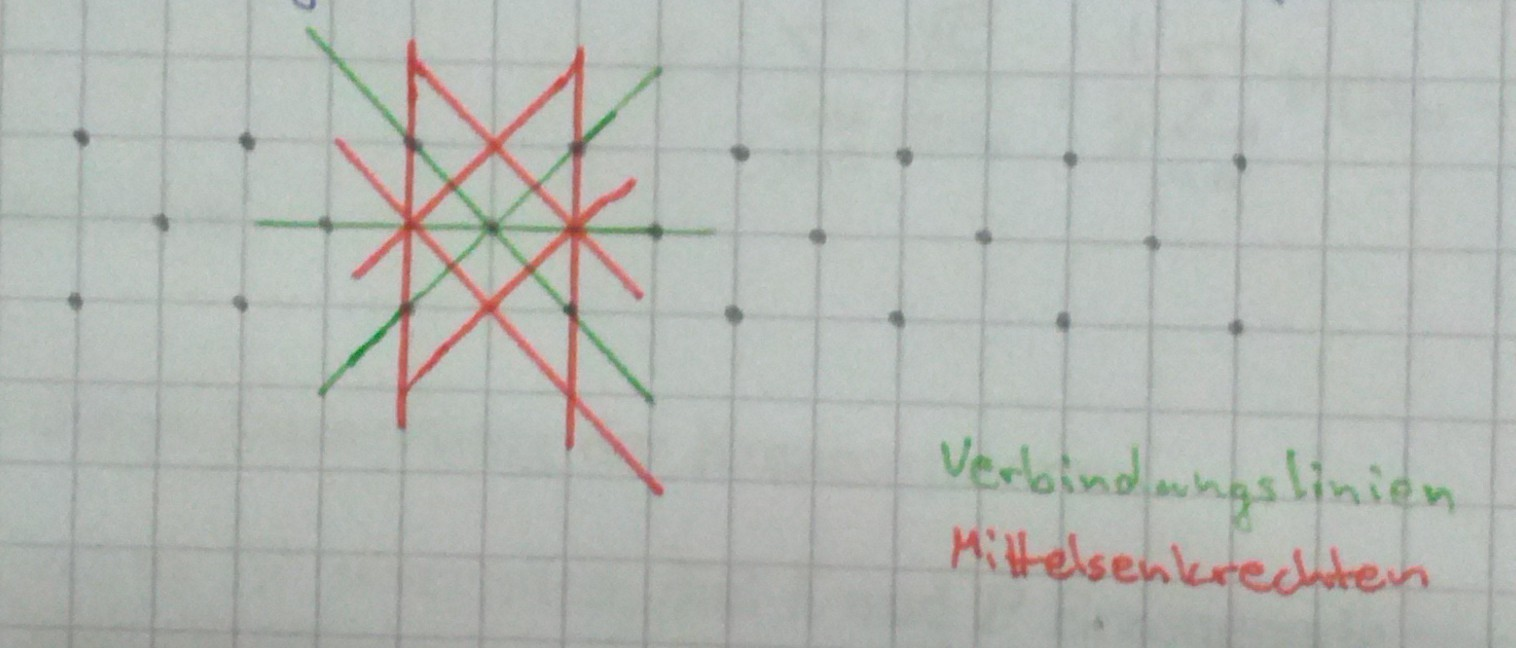
\includegraphics[width=0.6\textwidth]{pics/pic002.jpg}
				%\caption{}
			\end{figure}
			Jeder Gitterpunkt kann mit einer Basis von Atomen besetzt 
			werden.
			\begin{center}
				\fbox{Kristallstruktur = Gitter + Basis}
			\end{center}
			\begin{figure}[H]
					\centering
					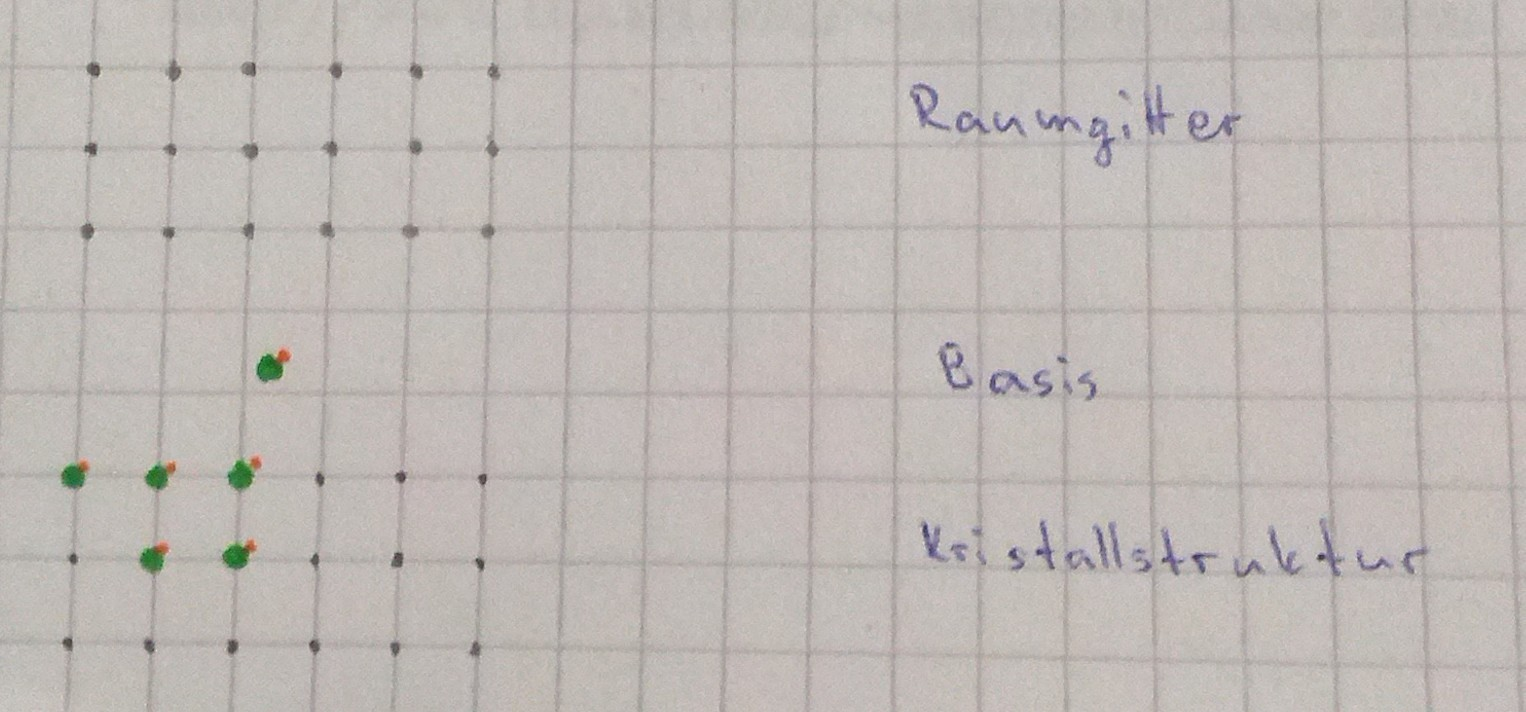
\includegraphics[width=0.6\textwidth]
					{pics/pic003.jpg}
					%\caption{}
			\end{figure}
				Ein Kristall zeichnet sich durch seine \emph{Symmetrien} 
				aus:
			\begin{itemize}
				\item Translationen (s.o.)
				\item Spiegelungen
				\item Drehsymmetrien
			\end{itemize}
			\emph{Definition}: Eine Drehachse, bei der der Kristall nach 
			Drehung um den Winkel $\nicefrac{2\pi}{n}$ 
			($n \in \mathbb{N}$) in sich selbst übergeht, heißt 
			\emph{n-zählige Drehachse}\\
			\emph{Behauptung}: $n=1, 2, 3, 4, 6$; sonst keine Werte 
			möglich\\
			\emph{Beweis}: 
			\begin{figure}[H]
					\centering
					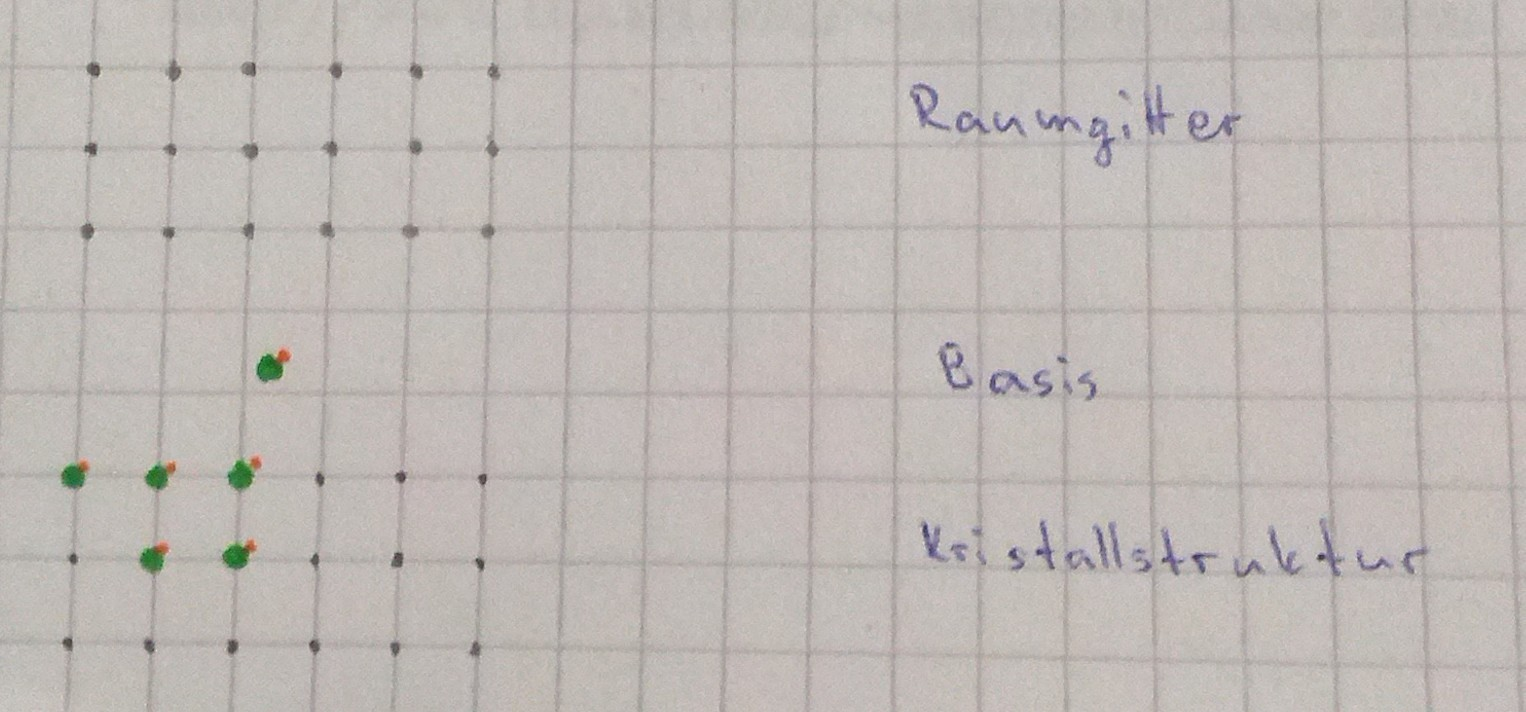
\includegraphics[width=0.6\textwidth]
					{pics/pic003.jpg}
					%\caption{}
			\end{figure}
			\begin{align*}
				&\vec{a}=\left( \begin{smallmatrix} 1 \\ 0 
				\end{smallmatrix}
				\right)	\;\text{ist Translationsvektor}\\
				&\begin{rcases}
					a_+ = \left( \begin{smallmatrix} \cos 
					(\nicefrac{2\pi}{n}) \\ \sin (\nicefrac{2\pi}{n}) 
					\end{smallmatrix} \right)\\
					a_- = \left( \begin{smallmatrix} \cos 
					(\nicefrac{2\pi}{n}) \\ -\sin (\nicefrac{2\pi}{n}) 
					\end{smallmatrix} \right)\\
				\end{rcases}
				\begin{array}{l}
					\text{ist ein blablabla}\\
					\text{aber auch ein blablabla}
				\end{array}
			\end{align*}
			$\Rightarrow$ auch $\vec{a_+}+\vec{a_-}$ ist ein 
			Gittervektor $=a \left( \begin{smallmatrix} \cos 
			(\nicefrac{2\pi}{n})\\ 0 \end{smallmatrix} \right)$. Wenn 
			$\vec{a}$ kleinster Translationsvektor ist, muss gelten
			\begin{align*}
				\vec{a_+}+\vec{a_-} = m \vec{a}; m \in \mathbb{Z}\\
				\Rightarrow \boxed{\underbrace{2\cos 
				(\nicefrac{2\pi}{n})}_{\text{\normalfont Wann ist dies 
				eine ganze Zahl?}} = m}	
			\end{align*}
			\emph{graphisch}:
			\begin{figure}[H]
				\centering
				\begin{minipage}[c]{0.6\textwidth}
					\centering
					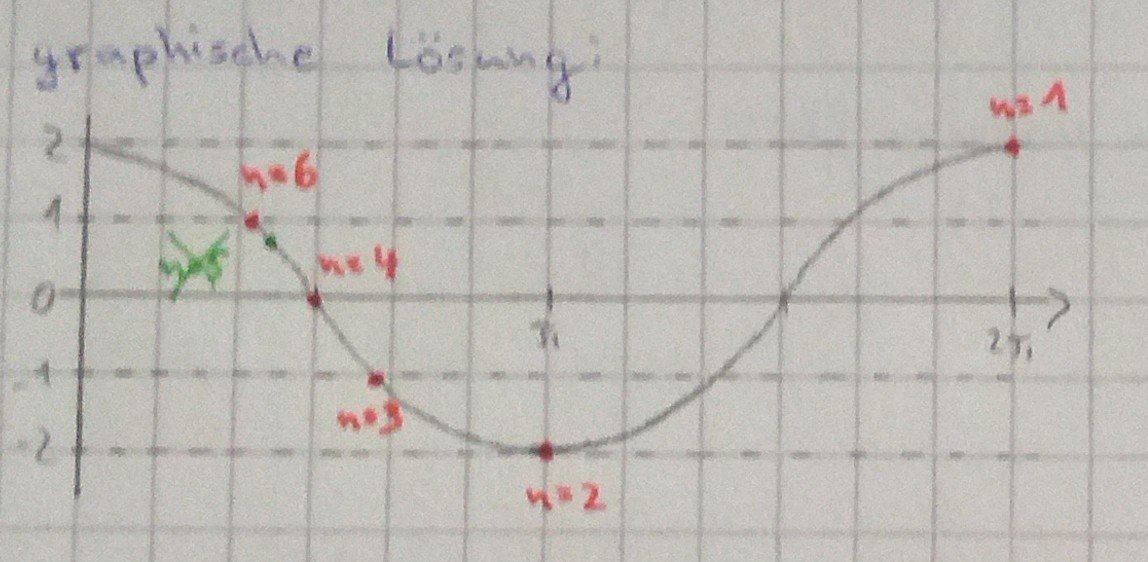
\includegraphics[width=0.9\textwidth]
					{pics/pic005.jpg}
				\end{minipage}	
				\begin{minipage}[c]{0.39\textwidth}
					\centering
					\begin{tabular}{cc}
						\toprule
						$n$ & $2 \cos (\nicefrac{2\pi}{n})$ \\
						\midrule
						1	&	2	\\
						2	&	-2	\\
						3	&	-1	\\
						4	&	0	\\
						5	&	0,61\\
						6	&	1	\\
						7	&	1,25\\
						\vdots & \vdots\\
						\bottomrule
					\end{tabular}
				\end{minipage}	
			\end{figure}
			$\Rightarrow$ $n \in {1, 2, 3, 4, 6}$ q.e.d.\\
			
			In 3D existieren 14 verschiedene Raumgitter, die man als 
			\emph{Bravais-Gitter} bezeichnet.
			Diese können in sieben verschiedene \emph{Kristallsysteme} 
			eingeordnet werden.
			
			BILD POWERPOINTFOLIE

\marginpar {29.10.2013}	

			Häuufig möchte man Netzebenen bzw. Netzebenenscharen kennen.
			$\Rightarrow$ Miller'sche Indizes
			
			\emph{Definition}: Gegeben seien die Kristallachsen 
			$\vec{a_1}$, $\vec{a_2}$, $\vec{a_3}$ (nicht unbedingt 
			kartesisch, nich unbedingt primitiv). Die Ebene sei 
			aufgespannt durch die drei Vektoren $n_{1}\vec{a_1}$, 
			$n_{2}\vec{a_2}$, $n_{3}\vec{a_3}$; $n_{1}, n_{2}, n_{3} 
			\in \mathbb{N}$
			
			BILD
			
			Die (kleinsten) ganzen Zahlen, die sich verhalten wie die 
			Kehrwerte von n1, n2, n3 bilden die Miller'schen Indizes.
			\emph{Beispiel}: $\left( \frac{1}{2}, \frac{1}{3}, 
			\frac{1}{1} \right) \Rightarrow (3,2,6)$ FEHLT WAS Meist 
			lässt man die Kommata weg, also "$(326)$". Negative Werte 
			werden druch Balken dargestellt, also z.B 
			$(32\overline{6})$. Wird eine Achse nicht geschnitten (ist 
			also der Achsenabschnitt = $\inf$), so ist der zugehörige 
			Miller'sche Index $=0$. 
			\emph{Beispiel}:
			
			BILD BILD
			
		\subsubsection{Einfache Kristallstrukturen und ihre Bindung}
			Natriumchloridstruktur:
				\addmargin{1cm}
				\emph{Beispiel}: NaCl, KCl, MnO, KBr, $\ldots${}\\
				\emph{Bravais-Gitter}: kubisch flächenzentriert (fcc)\\
				\emph{Basis}: ein Na und ein Cl (beim NaCl)
				\emph{Bindung}: ionisch
				\addmargin{-1cm}
				Na hat die Elektronenkonfiguration $1s^{2}2s^{2}2p^{6}3s^{1}$
				Cl $1s^{2}2s^{2}2p^{6}3s^{2}3p^{5}$
				$\Rightarrow$ gibt das Na ein Elektron an das Cl ab, so 
				weisen beide abgeschlossene Schalen auf. Es entsteht ein Na$^{+}$
				und Cl$^{-}$ Ion, die sich auf Grund der Coulombkraft anziehen\\
				
				Wir betrachten \emph{$N=N_{A}$} Ionenpaare. Es v die Coulombenergie
				\begin{align*}
					U^{c} = N \sum_{j, j\not i} \frac{\pm e^{2}}{4\pi \epsilon_{0} r_{ij}}\\
					+ \text{entspricht Abstoßung Na$^{+}$}Na$^{+}$} (i in Na$^{+}$} gewählt)\\
					- \text{entspricht Anziehung Na$^{+}$}Cl$^{-}$}}
				\end{align*}
				Mit der Definition $r_{ij} :\= p_{ij}r_{0}$, $r_{0}$ ist der Abstand nächster Nachbarn wird 
				hieraus
					\begin{align*}
						U^{c} = \frac{Ne^{2}}{4\pi\epsilon_{0}r_{0}}\underbrace{\sum_{j, j nicht i} \frac{\pm 1}{p_{ij}}_{:= -\alpha}
					\end{align*}
				$[\alpha] = 1$, $\alpha > 0$ sonst $U^{c} > 0$
				
				
				\emph{Beispiel}: (1D Kette)
				BILD
				
				$\alpha = 2\left( \frac{1}{1} - \frac{1}{2} + \frac{1}{3} - \frac{1}{4} + \frac{1}{5} \ldots${}
				mit $\ln (1+x) =x - \frac{x^{2}}{2} + \frac{x^{3}}{3} - \frac{x^{4}}{4} + \frac{x^{5}}{5} \ldots $
				
				
				In 3D ist die Summation im Allgemeinen \emph{viel} schwieriger. Die Reihen konvergieren oft schlecht $\Rightarrow${}
				"geschickte" umgruppierung der Summanden\\
				
				\emph{Beispiel}: (NaCl)
				\begin{tabular}{cc}
					\toprule{}
					Ionen		&	Abstand		\\
					\midrule{}
					Na$^{+}$	&	0			\\
					6Cl$^{-}$	&	$r_{0}$		\\
					12Na$^{+}$	&	$\sqrt{2}r_{0}$\\
					8Cl$^{-}$	&	$\sqrt{3}r_{0}$\\
					6Na$^{+}$	&	$\sqrt{4}r_{0}$\\
					\vdots		&	\vdots{}
					\bottomrule
				\end{tabular}
				$\Rightarrow \alpha = \frac{6}{1} - \frac{12}{\sqrt{2} + \frac{8}{\sqrt{3} - \frac{6}{\sqrt{4} = 1,7475$\\
				$\sum = $
				
				Es existiert auch eine Abstoßende wechselwirkung auf Grund der überlappenden Elektronenhüllen
				und des \emph{Pauliverbots}. Dies ist ein quantenmechanischer Effekt. Man setzt \emph{phänomenologisch} an
				\begin{align*}
					U_{i}^{B} = +Be^{\nicefrac{r_{ij}}{\rho}}
				\end{align*}
				KASTEN DRUM CAPTOPN: Born-Mayer-Potential
				$B$ und $\rho$ sind materialspezifische Konstanten. Summation also nur über nächte Nachbarn (NN)
				\begin{align*}
					U^{B} = N \cdot z \cdot B \cdot e^{\nicefrac{r_{ij}}{\rho}}\\
					N: Zahl der Ionenpaare, auch "Koordinationszahl", z.B. Na$^{+}$ hat $n = 6$					
				\end{align*}
				Die gesamte Energie ist 
				\begin{align*}
					U = U^{C} + U^{B}\\
					\Rightarrow U = -N \left( \frac{e^{2}}{4\pi\epsilon_{0}}\alpha - z\cdot Be^{\nicefrac{r_{0}}{\rho}}
				\end{align*}
				\emph{graphisch}:
				BILD
				
				Gleichgewichtslage bei $\frac{dU}{dr_{0}}=0$
				\begin{align*}
					\Rightarrow 0 = -N \left( \frac{-e^{2}}{4\pi\epsilon_{0} r_{0}^{2}}\alpha - zB(1/\rho)e^{\nicefrac{r_{0}}{\rho}}\\
					\Rightarrow zBe^{\nicefrac{r_{0}}{\rho}} = \frac{\rho}{r_{0}}\frac{-e^{2}}{4\pi\epsilon_{0} r_{0}}
				\end{align*}
				Einsetzten:
				\begin{align*}
					\Rightarrow U = \frac{-Ne^{2}}{4\pi\epsilon_{0}r_{0}}\alpha \left( 1 - \frac{\rho}{r_{0}}
				\end{align*}
				Die Bindungsenergie pro Ionenpaar N ist 
				\begin{align*}
					E_{B} := \frac{U}{N}
				\end{align*}
				\emph{Beispiel}: (NaCl)
				r_{0} = 0,28nm
				\rho = 0,03nM
				klammer dahinter ->
				
			Cäsiumchlorid:
				\addmargin{1cm}
				\emph{Beispiel}: CsCl, CnPd, AlNi, AgMg, $ldots$
				\emph{Bravais-Gitter}: einfach kubisch
				\emph{Basis}: ein Cs und ein Cl
				\emph{Bindung}: ionisch
				Cs hat Elektronenkonfiguration ....6s^{1}
				Cl hat Elektronenkonfiguration .... 3p^{5}
				\Rightarrow analog zum NaCl
				
\end{document}
